\chapter{Estensione: assegnamenti, ambienti, sequenze}

\section{Assegnamento}
Ogni linguaggio di programmazione introduce le nozioni di \textbf{variabili} e \textbf{assegnamento}.

L'assegnamento non è una uguaglianza o equazione, ma denota l'azione di prendere la destra dell'uguale e metterla all'interno della sinistra dell'uguale, considerando come valori le variabili sulla destra e contenitori le variabili sulla sinistra.

Si deduce che il simbolo di variabile ha significato diverso tra la destra e la sinistra dell'operatore.

\subsection{L-Value vs R-Value}
Si definisce quindi la distinzione tra l-value e r-value:
\begin{itemize}
    \item \textbf{l-value}: il significato della variabile a sinistra è la variabile \textit{in quanto tale}
    \item \textbf{r-value}: il significato della variabile a destra è il \textit{contenuto} della variabile
\end{itemize}

Sorge inoltre la questione dell'\textit{assegnamento distruttivo/non distruttivo}, è possibile cambiare il valore associato in precedenza a un simbolo di variabile?

Nei linguaggi \textit{imperativi} l'assegnameto è distruttivo, nei linguaggi \textit{logici} si ha una trasparenza referenziale dove un simbolo ha sempre lo stesso valore.

\section{Environment}
Per esprimere al meglio la semantica dell'assegnamento, occorre introdurre il concetto di \textbf{environment}, inteso come \textit{insieme di coppie} \texttt{(simbolo, valore)}, esprimibile tramite una tabella a due colonne (\textbf{map}).

\begin{figure}[H]
    \caption{Mappa ambiente}
    \centering
    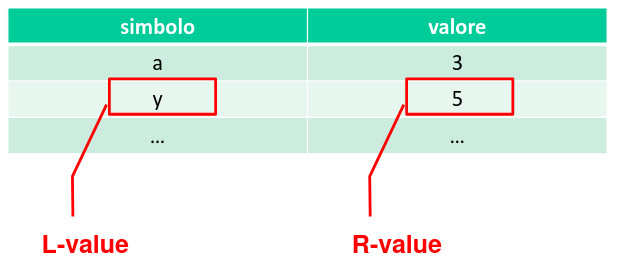
\includegraphics[width=0.7\textwidth]{/home/riccardoob/appunti/linguaggi/images/43.png}
\end{figure}

\subsection{Semantica}
Un assegnamento modifica l'environment causando un \textit{effetto collaterale} secondo questa semantica
\begin{equation*}
    \text{x} = \text{valore}
\end{equation*}

\begin{itemize}
    \item Se \textit{non esiste} una coppia adatta, se ne inserisce una nuova
    \item se \textit{esista} una coppia adatta, si denotano due possibilità
    \begin{itemize}
        \item \textbf{assegnamento distruttivo}: viene sostituita la coppia esistente con la nuova
        \item \textbf{singolo assegnamento}: viene mantenuta la coppia esistente, tentativi di assegnamento a x danno luogo a errori.
    \end{itemize}
\end{itemize}

\subsection{Environment multipli}

Nei linguaggi imperativi l'assegnamento è distruttivo, produce effetti \textit{collaterali} nell'environment.

Solitamente l'environment è suddiviso in sotto-ambienti collegati al \textit{tempo di vita} delle strutture run-time:
\begin{itemize}
    \item \textbf{environment globale}: coppie il cui tempo di vita è l'\textit{intero programma}
    \item \textbf{environment locale}: coppie con tempo di vita diverso dall'intero programma, tipicamente relativo a \textit{funzioni o altre strutture}.
\end{itemize}

Ogni modello computazionale deve specficiare il campo di \textit{visibilità dei suoi \textbf{simboli}}, ossia quali environment sono visibili in un certo punto del programma.

\section{Scelta del tipo di assegnamento}
É necessario valutare vari aspetti di un per l'introduzione di un sistema di assegnamento:
\begin{itemize}
    \item la sintassi dei nomi delle variabili
    \item se l'assegnamento sia \textit{distruttivo} o \textit{meno}
    \item decidere se la scrittura di assegnamento \texttt{x = valore} sia
    \begin{itemize}
        \item \textbf{istruzione}: effettua una azione senza denotare un valore
        \item \textbf{espressione}: effettua una azione e denota il valore risultante
    \end{itemize}
\end{itemize}

\subsubsection{Assegnamento multiplo}
Questa ultima considerazione dipende dal fatto che si voglia o meno supportare l'assegnamento multiplo, che consiste nel rendere valide espressioni come \texttt{x = y = z = valore}.

Normalmente l'assegnamento ha la natura di istruzione, in quanto causa un effetto collaterale nell'environment, tuttavia in questo modo si rende impossibile comporre assegnamenti multipli.

Consentire l'assegnamento multiplo implica interpretarlo come espressione, questo rende l'operatore di assegnamento \textit{associativo a destra}, poice il valore è l'ultimo elemento.
\begin{equation*}
    \texttt{x = (y = (z = valore))}
\end{equation*}

\subsection{Estensione dell'interprete}
Per implementare l'assegnamento occorre aggiungere la nozione di:
\begin{itemize}
    \item espressione di \textbf{assegnamento}, nuova \texttt{AssignExp} (produzione per EXP)
    \item \textbf{variabile} nelle sue due interpretazioni (L/R-value) che necessita di decidere se mantenenere la stessa sintassi per R e L-value, nuovo tipo di fattore (produzione per FACTOR)
\end{itemize}

Senza un simbolo che distingua R-value da L-value, la grammatica diventa LL(2).

Si aggiungono le produzioni:
\setlist{nosep}
\begin{itemize}[label={}]
    \item $P = \{$
    \begin{itemize}[label={}]
        \item $\dots$
        \item $\texttt{EXP} := \texttt{ASSIGN}$
        \item $\texttt{ASSIGN} := \texttt{IDENT} = \texttt{EXP}$
        \item $\texttt{FACTOR} := \$\texttt{IDENT}$
        \item $\texttt{IDENT} := \texttt{lettera}$
        \item $\dots$
    \end{itemize}
    \item $\}$
\end{itemize}
\setlist{}

Occorre inoltre estendere la sintassi astratta, si hanno tre nuovi tipi di nodo per l'AST:
\begin{itemize}
    \item nodo \textit{operazione assegnamento} $\rightarrow$ \texttt{AssignExp}
    \item nodo \textit{L-value} (\texttt{IDENT} a sinsitra) $\rightarrow$ \texttt{LIdentExp}
    \item nodo \textit{R-value} (\texttt{IDENT} a destra) $\rightarrow$ \texttt{RIdentExp}
\end{itemize}

In modo informale, si può definire il nodo L-value in modo da accedere al contenitore avente quel simbolo, e il nodo R-value in modo da ottenere il valore associato a quel simbolo nell'environment corrente.

\begin{figure}[H]
    \caption{Nuovi nodi}
    \centering
    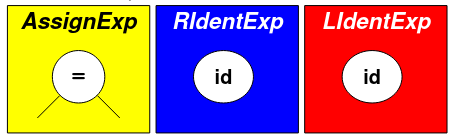
\includegraphics[width=0.6\textwidth]{/home/riccardoob/appunti/linguaggi/images/44.png}
\end{figure}

\begin{figure}[H]
    \caption{Nuova struttura delle classi}
    \centering
    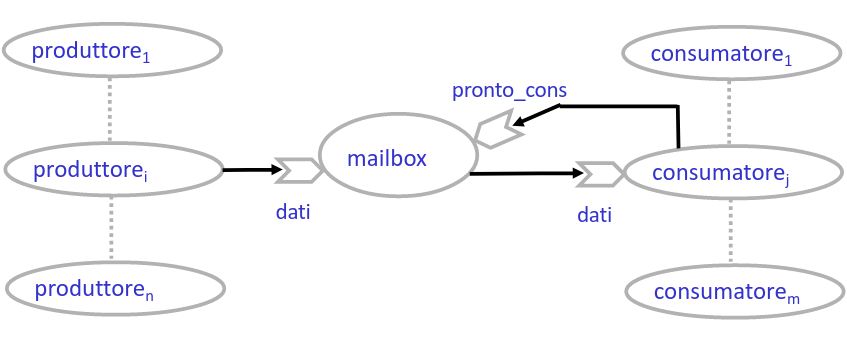
\includegraphics[width=0.7\textwidth]{/home/riccardoob/appunti/linguaggi/images/45.png}
\end{figure}

Nel parser si effettuano alcune modifiche per integrare comdodamente i nuovi nodi:
\begin{itemize}
    \item classe \texttt{Token} ha metodo \texttt{isIdentifier()} che controlla la sintassi degli identificatori
    \item \texttt{parseExp} cattura la nuova espressione \texttt{Assign} intercettando la sequenza $\texttt{IDENT} = \texttt{EXP}$
    \item \texttt{parseFactor} cattura il nuovo fattore \texttt{RIdent}, intercettando la sequenza $\$\texttt{IDENT}$
\end{itemize}


\textbf{\_\_\_\_\_\_\_\_\_\_\_\_\_\_\_\_\_\_\_\_\_\_\_\_\_\_\_\_\_\_\_\_\_\_\_\_\_\_\_\_\_\_\_\_\_\_\_\_\_\_\_inserisci codice slide 26-41\_\_\_\_\_\_\_\_\_\_\_\_\_\_\_\_\_\_\_\_\_\_\_\_\_\_\_\_\_\_\_\_\_\_\_\_\_\_\_\_\_\_\_\_\_\_\_\_\_\_\_}

\section{Espressioni sequenza}
Il prossimo obiettivo è quello di aggiungere la possibilità di esprimere più espressioni in sequenza, ovvero espressioni concatenate da una virgola.

Ipotizzando che la prima espressione è sempre un assegnamento e i valore complessivo è quello dell'exp più a destra:
\begin{itemize}[label={}]
    \item $\texttt{EXP} := \texttt{ASSIGN}, \texttt{EXP}$
\end{itemize}

Si indentifica il nuovo nodo \texttt{SeqExp}.
\begin{figure}[H]
    \centering
    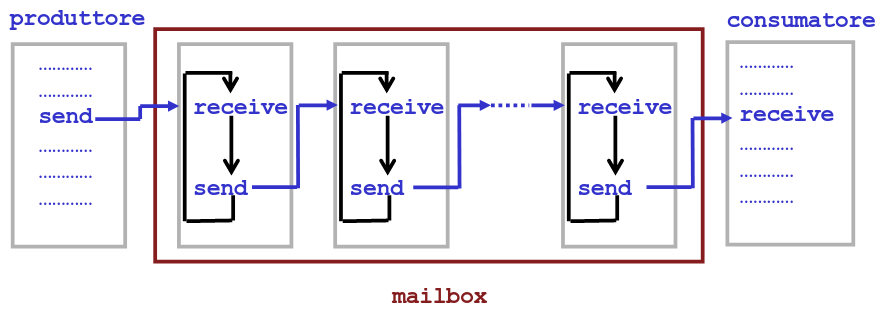
\includegraphics[width=0.2\textwidth]{/home/riccardoob/appunti/linguaggi/images/46.png}
\end{figure}

continua slide 47..


\textbf{\_\_\_\_\_\_\_\_\_\_\_\_\_\_\_\_\_\_\_\_\_\_\_\_\_\_\_\_\_\_\_\_\_\_\_\_\_\_\_\_\_\_\_\_\_\_\_\_\_\_\_inserisci codice slide 49-55\_\_\_\_\_\_\_\_\_\_\_\_\_\_\_\_\_\_\_\_\_\_\_\_\_\_\_\_\_\_\_\_\_\_\_\_\_\_\_\_\_\_\_\_\_\_\_\_\_\_\_}








































